\icode{N21E-EME-MU-L3-261121-001}
\nceeID[4]{2021湖北}{19}
（多选）
如图所示，一匀强电场\(E\)大小未知、方向水平向右。两根长度均为\(L\)的绝缘轻绳分别将小球\(M\)和\(N\)悬挂在电场中，悬点均为\(O\)。两小球质量均为\(m\)、带等量异号电荷，电荷量大小均为\(q\)（\(q>0\)）。平衡时两轻绳与竖直方向的夹角均为\(\theta =\)\qty{45}{\degree}。若仅将两小球的电荷量同时变为原来的2倍，两小球仍在原位置平衡。已知静电力常量为\(k\)，重力加速度大小为\(g\)，下列说法正确的是\paren[]

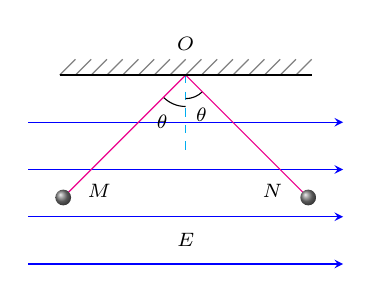
\begin{tikzpicture}[>=stealth,font=\scriptsize]
	\draw[dashed,cyan] (0,0)--(0,-1);
	\draw (0,-.3) arc(-90:-45:.3) (0,-.4) arc(-90:-135:.4);
	\foreach \y in {-2.4,-1.8,...,-.4}
		\draw[->,blue] (-2,\y)--(2,\y);
	\draw[magenta] (0,0)--(-45:2.2) (0,0)--(-135:2.2);
	\shade[ball color=gray] (-45:2.2) circle(.1);
	\shade[ball color=gray] (-135:2.2) circle(.1);
	\foreach \x in {-1.6,-1.4,...,1.6}
		\draw[gray] (\x,0)--++(.2,.2);
	\draw[thick] (-1.6,0)--(1.6,0);
	\node at(-1.1,-1.47){\(M\)};
	\node at(1.1,-1.47){\(N\)};
	\node at(.2,-.5){\(\theta\)};
	\node at(-.3,-.6){\(\theta\)};
	\node at(0,-2.1){\(E\)};
	\node at(0,.4){\(O\)};
\end{tikzpicture}
\begin{choices}
	\item \(M\)带正电荷
	\item \(N\)带正电荷
	\item \(q = L\sqrt{\dfrac{mg}{k}}\)
	\item \(q = 3L \sqrt{\dfrac{mg}{k}}\)
\end{choices}
\begin{answer}
	BC\qquad 提示：
\end{answer}